\section{Approach}

\subsection{Baseline method}
We take an intuitive approach as our baseline, which we call the most frequent noun.act.
Given an action class $(subject, verb, object)$ where $subject$ and $object$ are both concepts, e.g., $(country, invade, country)$.
 $S_{verb}$ is the set of verb's synonyms in WordNet. Since an action triple doesn't provide adequate information for verb sense disambiguation,
we take all synsets as verb's synonyms. $NA_{verb}$ is the the set of all derivationally related words whose semantic field
(or lexical file name) in WordNet is noun.act of verbs in $S_{verb}$.
Finally, we take the synonyms of nouns in $NA_{verb}$ and the first-K with highest Wiktionary frequency are taken as our candidates.

\begin{align}
    S_{verb} & = \{{ v \in S_i | S_i \ synset \ of \ verb}\} \\
    NA_{verb} & = \{{ NA_i \ d.r.w.  \ of \ s_i | s_i \in S_{verb}}\} \\
    S_{noun} & = \{{ n \in S_i | S_i \ synset \ of \ noun, noun \in NA_{verb}}\}
\end{align}

\subsection{Retrieval based method}

Under the assumption that nouns in news titles are likely to be good candidates
for abstraction of action instances in the news bodies, we use a TF-IDF based retrieval method
to find the action-noun mapping.

\begin{figure}[!htp]
 \centering
 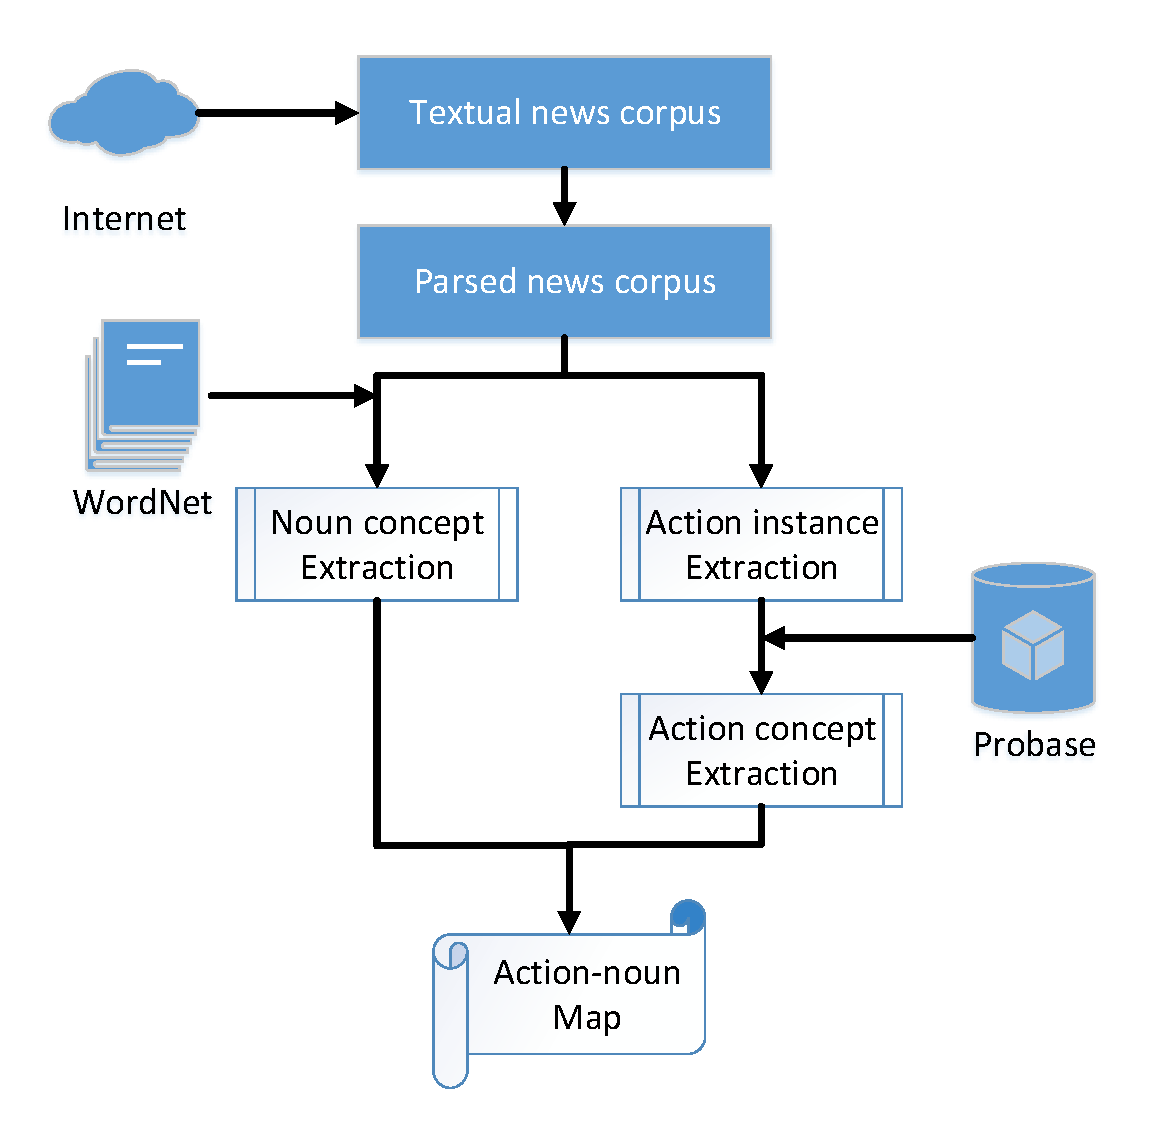
\includegraphics[width=\linewidth]{img/flow.pdf}
 \caption{Work flow}
\end{figure}

%% Some of the data.tex part should be moved to here.

We find the distribution of noun concepts in news titles, $f_n(i)$, and the distribution of action instances in news bodies,
denoted as $f_{ac}(i)$
\begin{align*}
    f_n(i) & = \{ j |  i \in t_j \} \\
    f_{ac}(i) &= \{ k | i \in b_k \}
\end{align*}
where $t_i$ and $b_i$ are title and body of $i^{th}$ news, respectively.

Next we use TFIDF to compute the relatedness of nouns to actions.
\begin{equation*}
    freq(n_i, ac_j) = \bigm| \{ k | n_i \in t_k \land ac_j \in b_k \} \bigm|
\end{equation*}
\begin{equation*}
    TF(n_i, ac_j) = \begin{cases} 0 &\mbox{if freq is 0} \\
        1 + log(freq(n_i, ac_j)) &\mbox{otherwise}
    \end{cases}
\end{equation*}


\begin{equation*}
    docfreq(n_i) = \bigm| \{ k | n_i \in t_k \} \bigm|
\end{equation*}


\begin{equation*}
    IDF(n_i) = log(\frac{\text{news corpus size}}{1 + docfreq(n_i)})
\end{equation*}

The result is for each action class, we have an array of noun concepts whose relatedness is represented by TF-IDF value with the action class.
\begin{figure}[!htp]
 \centering
 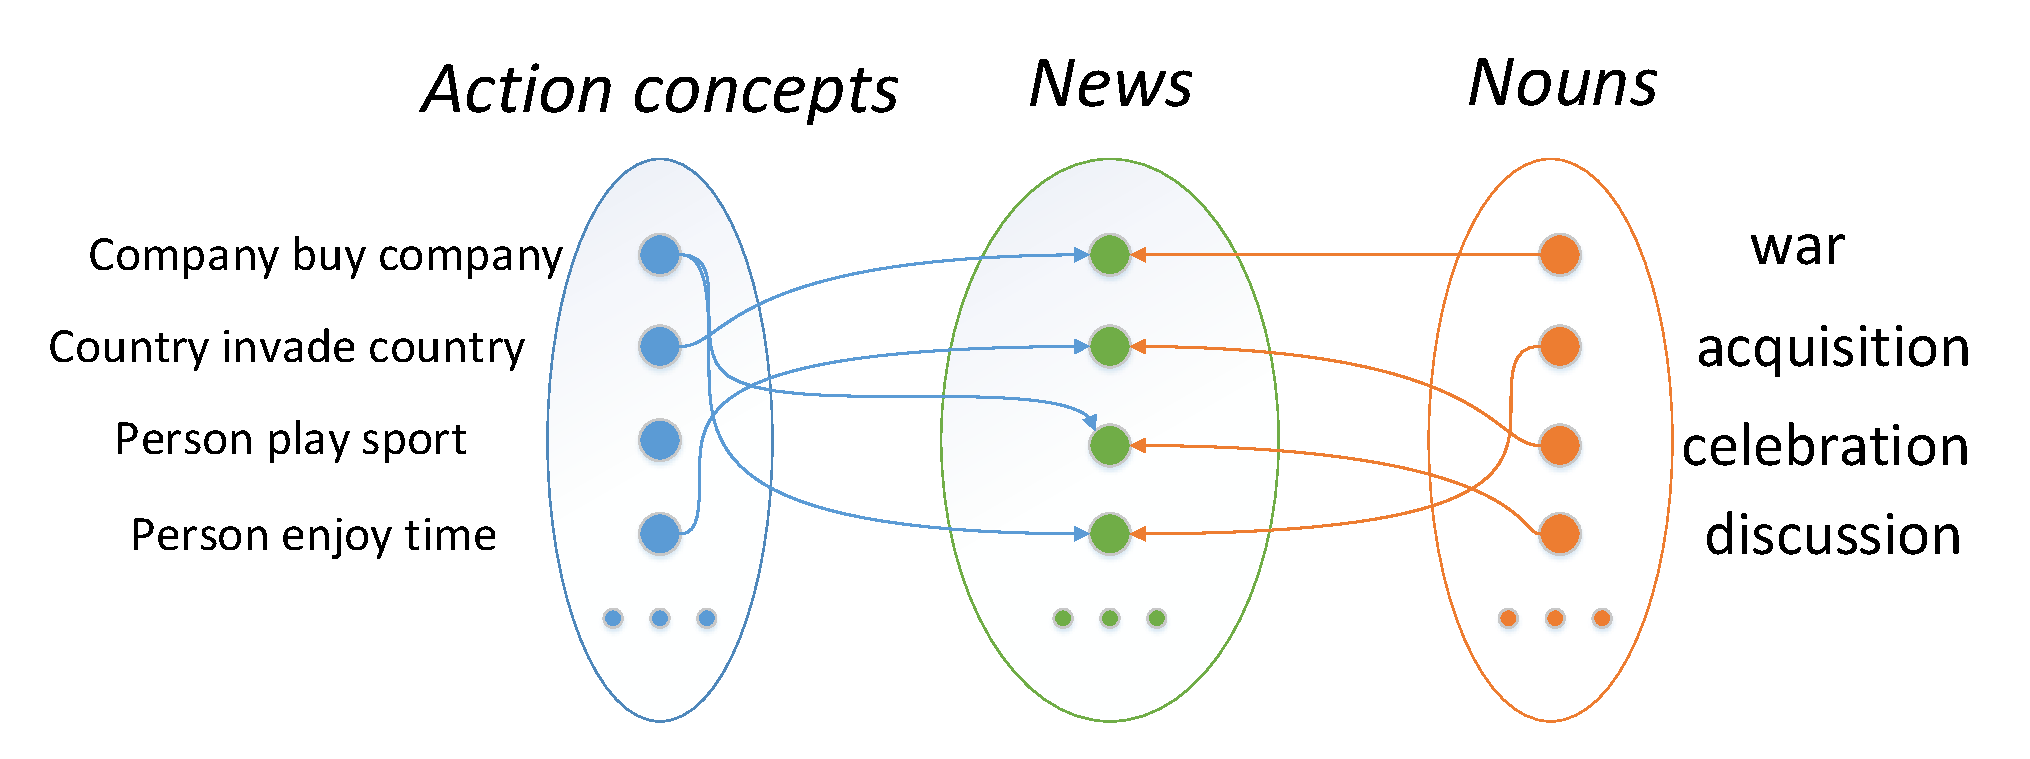
\includegraphics[width=\linewidth]{img/tripartite.pdf}
 \caption{Tripartite graph for construction of action-noun map}
\end{figure}
